\documentclass{beamer}
\usepackage[utf8]{inputenc}
\usepackage{pgfplots}
\usepackage{tikz}
\usepackage{hyperref}
\usepackage{geometry}
\usepackage{wasysym}
\usepackage{attrib}
\usepackage{float}
\usetikzlibrary{positioning,shapes,shadows,arrows,chains}
\usepackage{mathtools,amsfonts,amssymb}
\usepackage{graphicx}
\usetheme{Singapore}
\setbeamertemplate{footline}
{%
    \begin{beamercolorbox}{author in head/foot}
        \insertshortauthor \hfill \insertsubtitle \hfill \insertframenumber / \inserttotalframenumber
    \end{beamercolorbox}%
}
\setbeamertemplate{navigation symbols}{} % remove navigation symbols

\begin{document}

\title{Selbstorganisierte Kritikalität}
\subtitle{Proseminar für Chaos, Musterbildung und Selbstorganisation}
\date{2014-07-10}
\author{Sven-Hendrik Haase}
\institute{Universität Hamburg, Fakultät für Informatik}

\begin{frame}
    \titlepage
\end{frame}

\begin{frame}{Übersicht}
    \tableofcontents
\end{frame}

\section{Leitfragen}
\begin{frame}{\insertsection}{\insertsubsection}
	\begin{quote}
        ``Ausgedehnte Systeme neigen dazu, von selbst einen kritischen Zustand zu entwickeln,
        welcher fern vom Gleichgewicht liegt.''
        \tiny
        \attrib{übersetzt aus Physical Review Letters Vol 59, Number 4, Self-Organized Criticality, Per Bak,
        Chao, Tang, Kurt Wiesenfeld}
	\end{quote}
    \pause
    \begin{itemize}
        \item Was bedeutet ``kritisch'' bzw. ``Kritikalität''?
        \pause
        \item Was bedeutet ``von selbst'' bzw. ``selbstorganisiert''?
        \pause
        \item Wie werden diese Erkenntnisse in der Physikangewandt?
        \pause
        \item Können diese Konzepte außerhalb der puren Wissenschaft angewandt werden?
    \end{itemize}
\end{frame}

\section{Einfuehrung}
\subsection{Teil 1}
\begin{frame}{\insertsection}{\insertsubsection}
	\begin{itemize}
		\item Self-organized criticality (SOC) ist ein Phänomen bei dynamischen Systemen mit
            räumlicher Unbeschränktheit
        \pause
        \item Mit der Zeit nähern sich die Parameter des dynamischen Systems von selbst einem
            \textbf{kritischen Punkt} an
        \pause
        \item An einem \textbf{kritischen Punkt} findet ein \textbf{Phasenübergang} statt
        \pause
        \item Bei einem \textbf{Phasenübergang} reicht eine geringfügige quantitative Änderung des Systems
            aus, um eine signifikante qualitative Änderung des Systems herbeizuführen
        \pause
        \item Der \textbf{kritische Punkt} ist ein Attraktor
	\end{itemize}
\end{frame}

\subsection{Teil 2}
\begin{frame}{\insertsection}{\insertsubsection}
	\begin{itemize}
		\item Komplexe Strukturen entstehen durch einfache lokale Interaktionen
        \pause
		\item Es ist momentan unmöglich vorherzusagen, ob ein Algorithmus oder System
            SOC-artiges Verhalten aufweist (Simulation erforderlich)
        \pause
        \item Entstehende Systeme sind gerade noch stabil
        \pause
        \item Es kommt nicht so sehr auf die Anfangsparameter an (\textbf{selbst}organisiert)
        \item Anfangsparameter können stark variiert werden, ohne dass sich Endzustand stark ändert
	\end{itemize}
\end{frame}

\section{Forschung}
\begin{frame}{\insertsection}{\insertsubsection}
    \begin{itemize}
        \item Forschung an dem Thema setzt sich aus drei Forschungszweigen zusammen:
        \begin{itemize}
            \item Fraktale
            \item zulluläre Automaten und emergente Strukturen
            \item Phasenübergänge
        \end{itemize}
        \pause
        \item Paper von Bak, Tang und Wiesenfeld 1987 vereinte diese Forschungen
        \pause
        \item SOC-Konzepte heute in vielen Feldern der Wissenschaft vorhanden: Geophysik,
                Kosmologie, Evolutionsbiologie, Ökologie, Bioinformatik, Optimierung, Ökonomie,
                Quantengravitation, Soziologie, Solarphysik, Plasmaphysik, Neurobiologie
    \end{itemize}
\end{frame}

\section{Beispiele}
\subsection{Anwendungen}
\begin{frame}{\insertsection}{\insertsubsection}
	\begin{itemize}
        \item Bak–Tang–Wiesenfeld–Modell für Lawinen (auch ``Sandpile Model'')
        \item Bak-Sneppen Modell für Evolution
        \item Drossel-Schwabl Modell für Waldbrände
        \item Olami–Feder–Christensen Modell für Erdbeben
        \pause
        \item Landformationen
        \item Boersendynamik
        \item Gehirnsignale
        \item Neutronensternbeben
        \item Solarflares
	\end{itemize}
\end{frame}

\subsection{Sandpile Model}
\begin{frame}{\insertsection}{\insertsubsection}
	\begin{itemize}
        \item Modell für Lawinen
        \item Zellulärer Automat auf einem beschränkten Raster
        \pause
        \item Funktionweise:
            \pause
            \begin{itemize}
                \item Zufällige oder zentrale Platzierung von Chips auf dem Raster
                \pause
                \item Anzahl der Chips pro Zelle geben die Steigung an
                \pause
                \item Übersteigt die Zahl der Chips eine Schwelle, teilt die Zelle ihre Chips auf ihre Nachbarn auf
            \end{itemize}
        \item \textbf{Video Simulation}
        \item \textbf{Video Experiment}
	\end{itemize}
\end{frame}

\begin{frame}{\insertsection}{\insertsubsection}
    \begin{figure}[p]
        \centering
        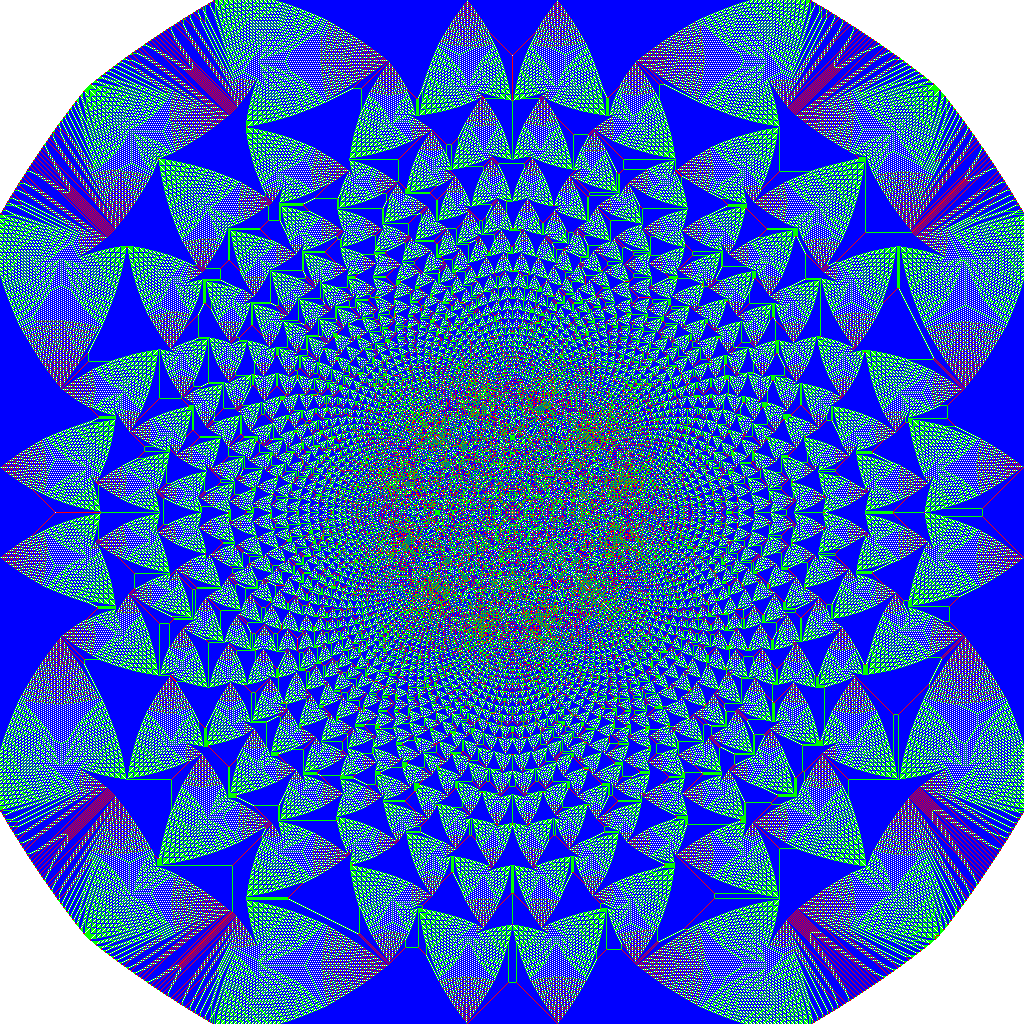
\includegraphics[scale=0.17]{Backtang2.png}
        \caption{Simulation von 28M Sandkörnern}
    \end{figure}
\end{frame}

\subsection{Bak-Sneppen Modell für Evolution}
\begin{frame}{\insertsection}{\insertsubsection}
	\begin{itemize}
        \item lol
	\end{itemize}
\end{frame}

\subsection{Drossel-Schwabl Modell für Waldbrände}
\begin{frame}{\insertsection}{\insertsubsection}
	\begin{itemize}
        \item lol
	\end{itemize}
\end{frame}

\subsection{Olami-Feder-Christensen Modell für Erdbeben}
\begin{frame}{\insertsection}{\insertsubsection}
	\begin{itemize}
        \item lol
	\end{itemize}
\end{frame}

\section{Quellen}
\begin{frame}{\insertsection}{\insertsubsection}
	\begin{itemize}
        \tiny
        \item \url{Bak, P., Tang, C. and Wiesenfeld, K. (1987). "Self-organized criticality: an
            explanation of 1/f noise". Physical Review Letters 59 (4): 381–384.}
        \item \url{https://www.youtube.com/watch?v=-d7\_OGn22d4}
        \item \url{https://www.youtube.com/watch?v=LfJCngN44ug}
        \item \url{http://commons.wikimedia.org/wiki/File:Backtang2.png}
	\end{itemize}
\end{frame}


\end{document}
